% Figure 1: generic hierarchical multi-agent self-protecting architecture.
% Compile standalone: pdflatex fig_architecture.tex -> fig_architecture.pdf
\documentclass[tikz,border=4pt]{standalone}
\usetikzlibrary{shapes.geometric,arrows.meta,positioning,calc}

\begin{document}
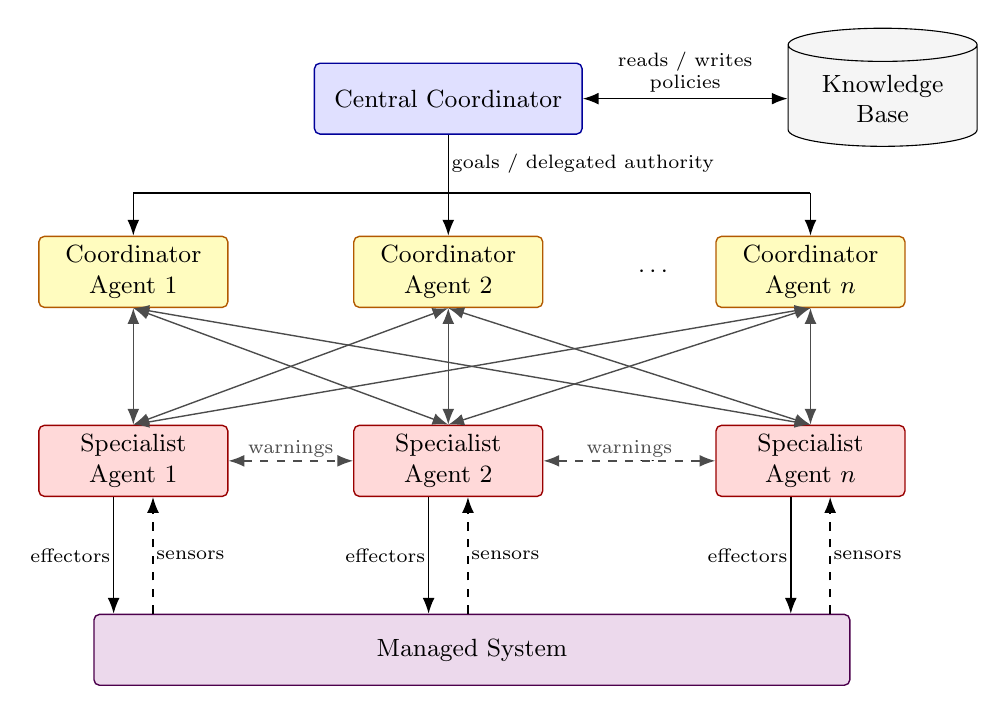
\begin{tikzpicture}[
  font=\small,
  box/.style={draw, rounded corners=2pt, minimum height=9mm, minimum width=24mm,
              align=center, line width=0.5pt},
  central/.style={box, fill=blue!12, draw=blue!60!black, minimum width=34mm},
  coord/.style={box, fill=yellow!25, draw=orange!70!black},
  spec/.style={box, fill=red!15, draw=red!60!black},
  managed/.style={box, fill=violet!15, draw=violet!60!black, minimum width=96mm, minimum height=9mm},
  kb/.style={cylinder, shape border rotate=90, draw, aspect=0.25, fill=gray!8,
             minimum height=15mm, minimum width=24mm, align=center, inner sep=2pt},
  flow/.style={-{Latex[length=2mm]}, line width=0.5pt},
  both/.style={{Latex[length=2mm]}-{Latex[length=2mm]}, line width=0.5pt},
  sensor/.style={-{Latex[length=2mm]}, line width=0.5pt, dashed},
  lbl/.style={font=\scriptsize, fill=white, inner sep=1pt, align=center}
]

% --- Central coordinator and knowledge base -------------------------------
\node[central] (cc) at (0,0) {Central Coordinator};
\node[kb, right=26mm of cc] (kb) {Knowledge\\Base};
\draw[both] (cc.east) -- node[lbl, above, yshift=1pt] {reads / writes\\policies} (kb.west);

% --- Coordinator agents ---------------------------------------------------
\node[coord] (c1) at (-4.0,-2.2) {Coordinator\\Agent 1};
\node[coord] (c2) at (-0.0,-2.2) {Coordinator\\Agent 2};
\node (cd)        at ( 2.6,-2.2) {$\cdots$};
\node[coord] (cn) at ( 4.6,-2.2) {Coordinator\\Agent $n$};

\coordinate (split) at (0,-1.2);
\draw[line width=0.5pt] (cc.south) -- node[lbl, right] {goals / delegated authority} (split);
\draw[line width=0.5pt] (-4.0,-1.2) -- (4.6,-1.2);
\foreach \c in {c1,c2,cn} { \draw[flow] (\c |- split) -- (\c.north); }

% --- Specialist agents ----------------------------------------------------
\node[spec] (s1) at (-4.0,-4.6) {Specialist\\Agent 1};
\node[spec] (s2) at (-0.0,-4.6) {Specialist\\Agent 2};
\node (sd)       at ( 2.6,-4.6) {$\cdots$};
\node[spec] (sn) at ( 4.6,-4.6) {Specialist\\Agent $n$};

\foreach \c in {c1,c2,cn} { \foreach \s in {s1,s2,sn} { \draw[both, gray!60!black] (\c.south) -- (\s.north); } }

% warnings between specialists (relayed by a coordinator)
\draw[both, dashed, gray!60!black] (s1.east) -- node[lbl, above] {warnings} (s2.west);
\draw[both, dashed, gray!60!black] (s2.east) -- node[lbl, above] {warnings} (sn.west);

% --- Managed system -------------------------------------------------------
\node[managed] (ms) at (0.3,-7.0) {Managed System};

\foreach \s in {s1,s2,sn} {
  \draw[flow]   ([xshift=-2.5mm]\s.south) -- node[lbl, left]  {effectors} ([xshift=-2.5mm]\s.south |- ms.north);
  \draw[sensor] ([xshift= 2.5mm]\s.south |- ms.north) -- node[lbl, right] {sensors} ([xshift=2.5mm]\s.south);
}

\end{tikzpicture}
\end{document}
